

\section{Klärung der Begrifflichkeiten}

\subsection{BMK-IoT Modul}
Das „BMK-IoT Modul“ ist ein Design In Modul. Eine bereits entwickelte Hardwaregrundlage mit Mikrocontroller, WLAN-Chip, eMMC und weiteren Schnittstellen, sowie fertigen Softwaregrundlagen im Bereich der Embedded Security, RTOS und Cloud ermöglichen der BMK-Entwicklung kundenspezifische Projekte schneller und einheitlicher zu realisieren.
Die dafür benötigte Hardware findet auf einer kleinen Platine mit BGA-Sockel Platz. 

\begin{center}
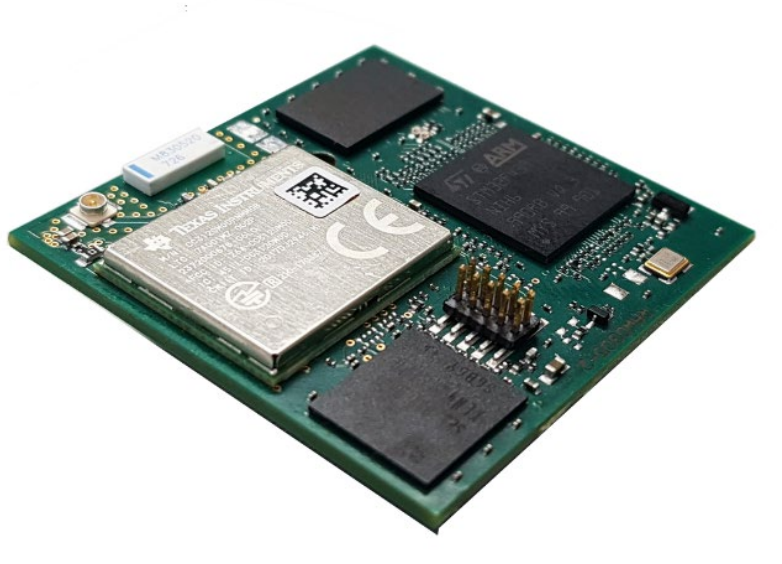
\includegraphics[width=10cm]{Bilder/BMK-IOT-MODUL.png}
\end{center}

\subsection{eMMC}
eMMC = embedded MultiMediaCard.
\\
Ein \glqq eMMC \grqq{} ist eine Variante eines Speicherkarten Standards. Durch seine preiswerte kompakte Größe wird diese Art häufig in mobile Endgeräte verbaut. Die verwendete Technologie ist die eines Flash-Speichers . Flash-Speicher und Flash-Controller werden auf dem selben Silizium-Chip integriert. Dabei sind Übertragungsraten bis zu 400MB/s möglich. eMMC's werden häufig direkt verlötet und sind deshalb ein Teil eines \glqq embedded System \grqq{}.


\subsection{RTOS}
RTOS = Real Time Operating System
\\
Ein \glqq Real Time Operating System \grqq{} besitzt die grundlegende Aufgabe, zu entscheiden welcher Task (Programmteil) wann ausgeführt wird. Für den Anwender, soll es dabei so aussehen, als ob die Anwendungen gleichzeitig abgearbeitet werden. In der Realität werden den Task's verschiedene Priorisierungen zugewiesen. Dadurch kann der Prozess-Scheduler entscheiden, welche Task wann und vor welchen anderen Task's abgearbeitet wird. 
\\
Nicht nur im Bereich des \glqq Event Handlings \grqq{} ist ein RTOS sehr wichtig, sondern auch im Bereich des Speicherzugriffes bieten sich RTOS-spezifische Funtionen an. Kommt es z.B. zu einem gleichzeitigen Speicherzugriff zweier Prozessorkerne, so kann es zu fatalen Fehlern kommen. Eine Priorisierung ist hier ebanfalls sehr wichtig.

\newpage
\subsection{BGA}
BGA = Ball Grid Array
\\
Unter \glqq BGA\grqq versteht man eine Art der Gehäuseform, wobei die Anschlüsse für die SMD-Bestückung auf der Unterseite des Bauteiles liegen. Kleine Lötperlen auf der Unterseite, können dabei durch einen Reflow-Prozess mit der Platine verlötet werden. Diese Technologie lässt dabei eine große Menge an Pin's auf einem kleinen Chip zu. 


\subsection{Pig-Tail}
Um bei hohen Frequenzen mit einem Oszilloskop bessere Messergebnisse zu erhalten, ist es oft hilfreich, ein Pig-Tail zu verwenden. Diese können oft beim Hersteller gekauft oder mit Silberdraht selbst gewickelt werden. 
\\
Das Messergebnis verbessert sich durch die niedrigere Induktivität der Masseleitung. Das über bzw. unterschingen des Messsignales verringert sich dadurch sichtbar. 


\begin{center}

\includegraphics[width=10cm]{Bilder/PigTail.jpg}


\end{center}


\begin{figure}[htb]
    \centering
    \begin{minipage}[t]{0.45\linewidth}
        \centering
        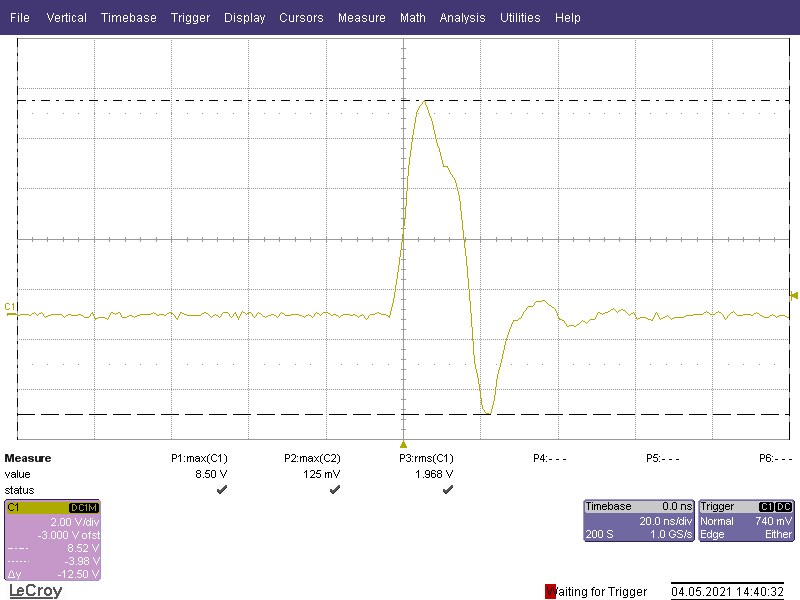
\includegraphics[width=8cm]{Bilder/TP19-ohne-PigTail.png}
        \caption{Signal ohne Pig-Tail}
    \end{minipage}% <- sonst wird hier ein Leerzeichen eingefügt
    \hfill
    \begin{minipage}[t]{0.45\linewidth}
        \centering
        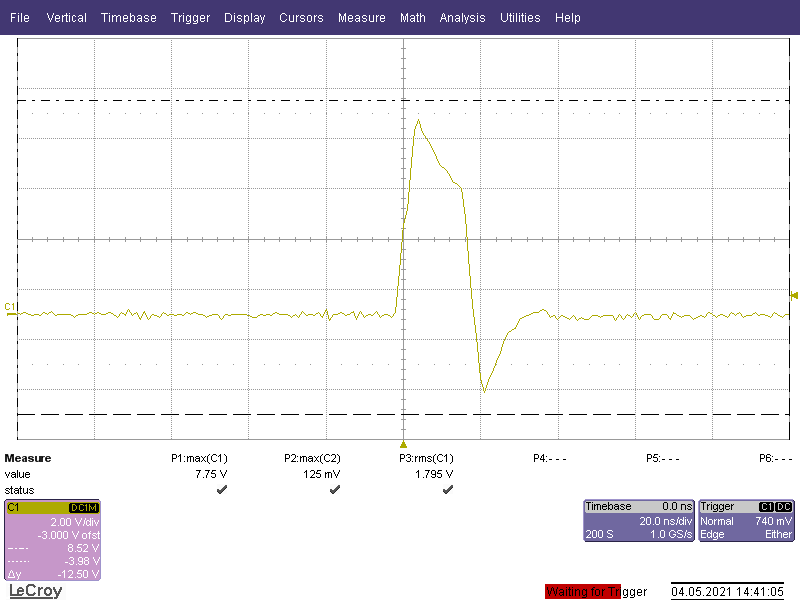
\includegraphics[width=8cm]{Bilder/TP19-mit-PigTail.png}
        \caption{Signal mit Pig-Tail}
    \end{minipage}
\end{figure}
